\section{Inclusion of the edge set in the construction}
\label{sec:edges}

%\subsection{Introduction}

The constructions from the previous section involve the vertex set $V$ and a group $\Gamma$ acting on it. Therefore, it looks natural to try to relate the edge set and $\Gamma$.

There are two point of views. Either $\Gamma$ describes an underlying graph structure $\gve$, either $G$ can be used to define a relevant subgroup $\Gamma$ to which the produced convolutive operators will be equivariant. Both approaches will help characterize classes of graphs that can support natural definitions of convolutions.

%\todo{introduction to be developped more}

%%
%% Draft
%%

%%% What follows is to be reworded and put in the neural network section !
% However we must keep in mind that the resulting convolution would be meant to breed a class of operators that are equivariant to $\Gamma$. In an application where this property is not relevant, such operators would produce layers that are less expressive than dense counterparts. So it is not always possible to leverage a graph structure coming with a dataset if one cannot build meaningful transformations from it. 

\subsection{Edge-constrained convolutions}
\label{sec:cayley}

% In this subsection, we are trying to answser the following question:
% \begin{itemize}
% 	\item What graphs admit a $\varphi$-convolution, or an $\M$-convolution , under the condition that $\Gamma$ is generated by a set of edge-constrained transformations ?
% \end{itemize}

\begin{definition}\textbf{Edge-constrained transformation}\\
An \emph{edge-constrained} (EC) transformation on a graph $\gve$ is a transformation $f: V \mapsto V$ such that
\begin{gather*}
\forall u,v \in V, f(u) = v \Rightarrow u \overset{E}{\sim} v
\end{gather*}
\end{definition}

\figref{fig:ec} gives a basic example of an EC transformation.

\begin{figure}[h!t]
    \begin{center}
      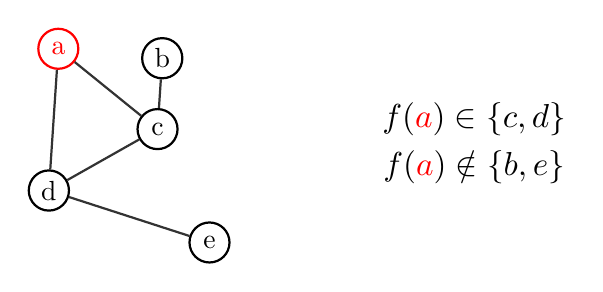
\begin{tikzpicture}[scale=0.6]
          \tikzstyle{every node} = [draw, circle, inner sep = 2pt, thick, minimum size=0.2in];
          \node(1) at (1,2) {d};
          \node[color=red](2) at (1.2,5) {\textcolor{red}{a}};
          \node(3) at (3.4,4.8) {b};
          \node(4) at (3.3,3.3) {c};
          \node(5) at (4.4,0.9) {e};
          \tikzstyle{every node} = []
          \path[opacity=0.8,thick]
          (1) edge (2);
          \path[opacity=0.8,thick]
          (2) edge (4);
          \path[opacity=0.8,thick]
          (4) edge (3);
          \path[opacity=0.8,thick]
          (1) edge (4);
          \path[opacity=0.8,thick]
          (1) edge (5);
          \tikzstyle{every node} = []
          \node at (10,3.5) {\scalebox{1.2}{$f(\textcolor{red}{a}) \in \{c,d\}$}};
          \node at (10,2.5) {\scalebox{1.2}{$f(\textcolor{red}{a}) \notin \{b,e\}$}};
          \end{tikzpicture}
    \end{center}
    \caption{Depiction of an EC transformation}
    \label{fig:ec}
  \end{figure}

We denote $\Phi_{\EC}(G)$ and $\Phi^*_{\EC}(G)$ the sets of EC and invertible EC transformations. Note that $\Phi^*_{\EC}(G)$ is not a group. Therefore, we are interested in generating sets of groups.

\begin{definition}\textbf{Edge-constrained convolution}\\
An \emph{edge-constrained} (EC) convolution on a graph $\gve$ is a $\varphi$- or $\M$-convolution of group $\Gamma$, such that $\Gamma$ is generated by a set $\cu$ which actions on $V$ are EC transformations.
\end{definition}

This leads us to consider Cayley graphs~\citep{cayley1878desiderata}.%,wiki:cayley}.

\begin{definition}\textbf{Cayley graph}\\
Let a group $\Gamma$ and one of its generating set $\cu$. The \emph{Cayley graph} generated by $\cu$, is the digraph $\vgve$ such that $V = \Gamma$ and $E$ is such that, either:
\begin{enumerate}[nolistsep,noitemsep,label=(\roman*)]
\item $\forall a,b \in \Gamma, a \rightarrow b \Leftrightarrow \exists g \in \cu, ga = b \quad$ (\emph{left Cayley graph})
\item $\forall a,b \in \Gamma, a \rightarrow b \Leftrightarrow \exists g \in \cu, ag = b \quad$ (\emph{right Cayley graph})
\end{enumerate}
We denote $\vec{G} = \langle \cu, \Gamma, E \rangle$. If $\Gamma$ is abelian, we call it an $\emph{abelian Cayley graph}$.
Also, we call \emph{Cayley subgraph} a directed subgraph that is isomorphic to a Cayley graph.
\end{definition}

\begin{remark}
Note that in the literature, a Cayley graph is usually what we defined as a right one. %However, we needed to also define left Cayley graphs since we made the choice to i
%In what follows, we could have used right Cayley graphs instead of left ones, but since we want $g$ to be an EC transformation, we would have had to use the right multiplicative action $g(a) = R_g(a) = ag$ and \eqref{eq:PPP} which is less convenient than \eqref{eq:P}. Recall that we made the choice to implicitly use left $\varphi$-equivalence unless stated otherwise.
\end{remark}

In the case of left Cayley graphs of vertex set $\Gamma$, it is clear that the $\varphi$-convolution based on $\Gamma$ is EC (since the $\varphi$-equivalence is implicitly under left multiplication).
More precisely, we obtain the following characterization:

\begin{theorem}\textbf{EC characterization by Cayley subgraphs}\\
Let a graph $\gve$,
\begin{enumerate}[nolistsep,noitemsep,label=(\roman*)]
\item its left Cayley subgraphs characterize its EC $\varphi$-convolutions,
\item its abelian Cayley subgraphs characterize its EC $\M$-convolutions.
\end{enumerate}
\label{th:cayleychar}
\end{theorem}

\begin{proof}
We show the result only in the first case since the proof in the abelian case is similar.
\begin{enumerate}
	\item Let an EC $\varphi$-convolution of group $\Gamma$. Since $\ast_\varphi$ is EC, there is a generating set $\cu$ such that its actions are EC.
  So the graph $\vec{G_s}$ defined such that $u \to v \Leftrightarrow \exists g \in \cu, g(u) = v$ is a subgraph of $G$, and we have:
  \begin{align*}
  u \to v & \Leftrightarrow \exists g \in \cu, g(u) = v\\
          & \Leftrightarrow \exists g \in \cu, g(\varphi(g_u)) = \varphi(g_v)\\
          & \Leftrightarrow \exists g \in \cu, \varphi(gg_u) = \varphi(g_v) \tag{since \eqref{eq:P}}\\
          & \Leftrightarrow \exists g \in \cu, gg_u = g_v
          %& \Leftrightarrow g_u \overset{G_c}\to g_v
  \end{align*}
  Therefore the subgraph $\vec{G_s}$ and the Cayley graph $\langle \cu, \Gamma, E_c \rangle$ are isomorphic via $\varphi$.

	\item Let a subgraph $\vec{G_s} = \langle V_s, E_s \rangle$ that is isomorphic to a left Cayley graph $\vec{G_c} = \langle \cu, \Gamma, E_c \rangle$. Let $\psi$ be a graph isomorphism from $G_s$ to $G_c$.%To obtain the proof, we need to find a group of invertible transformations $\Gamma$ of $V_s$ generated by a set of EC transformations, such that $\Gamma \equiv V_s$.

Let us define the group action $L : \Gamma \to \Phi^*(V_s)$ inductively as follows:
\begin{enumerate}[label=(\alph*)]
  \item $\forall g \in \cu, L_g(u) = v \Leftrightarrow g\psi(u) = \psi(v)$ \label{enum:a}
  \item Whenever $L_g$ and $L_h$ are defined, the action of $gh$ is defined by homomorphism as $L_{gh}= L_g \circ L_h$ \label{enum:b}
  \item Whenever $L_g$ is defined, the action of $g^{-1}$ is defined by homomorphism as $L_{g^{-1}}=L_g^{-1}$ \ie $L_{g^{-1}}(u) = v \Leftrightarrow \psi(u) = g\psi(v)$ \label{enum:c}
\end{enumerate}

Note that the induction transfers the property \ref{enum:a} to all $g \in \Gamma$ in a transitive manner because
\begin{gather*}
L_{gh}(u) = L_g(L_h(u)) = w \Leftrightarrow \exists v \in V_s
\begin{cases}
L_h(u) = v\\
L_g(v) = w
\end{cases}
\end{gather*}
and
\begin{gather*}
\exists v \in V_s
\begin{cases}
h\psi(u) = \psi(v)\\
g\psi(v) = \psi(w)
\end{cases}
\Leftrightarrow gh\psi(u) = \psi(w)
\end{gather*}

We must also verify that this construction is well-defined, \ie whenever we define an action with \ref{enum:b} or \ref{enum:c}, if the action was already defined, then they must be equal. This is the case because the homomorphism $g \mapsto L_g$ on $\Gamma$ is in fact an isomorphism as
\begin{align*}
L_g = L_h & \Leftrightarrow \forall u \in V, L_g(u) = L_h(u)\\
 & \Leftrightarrow \forall u \in V, g\psi(u) = h\psi(u)\\
 & \Leftrightarrow g = h
\end{align*}

Also note that \ref{enum:c} is needed only in case that $\Gamma$ is infinite.

Denote $\varphi = \psi^{-1}: g_u \mapsto u$ the inverse graph isomorphism. Since \ref{enum:a} has been transferred from $\cu$ onto $\Gamma$, we have, for all $g,h \in \Gamma$:
\begin{align*}
L_g(u) = v &\Leftrightarrow g\psi(u) = \psi(v)\\
           &\Leftrightarrow \varphi(g\psi(u)) = v\\
\ie L_g(u) &= \varphi(gg_u)
\end{align*}
So $\Gamma \overset\varphi\equiv V$. Furthermore, the corresponding $\varphi$-convolution is EC because of \ref{enum:a}.
\end{enumerate}
\end{proof}

\begin{remark}
Note that right $\varphi$-equivalences are instead characterized by right Cayley graphs.
\end{remark}

Through the former proof, we also obtain the following corollary. Note that we call an orientation $\vec{G_s} = \langle V_s, E_s \rangle$ of a graph $\gve$, a directed subgraph with same vertex set $V_s = V$ and such that $E_s \subset E$.

\begin{corollary}\textbf{$\varphi$ is a graph isomorphism from a Cayley graph}\\
Let a graph $\gve$, a group $\Gamma$ of generating set $\cu$ such that $\Gamma \overset\varphi\equiv V$. Then $\varphi$ is also a graph isomorphism between the left Cayley graph $\langle \cu, \Gamma, E_c \rangle$ and an orientation of $G$.
\label{cor:giso}
\end{corollary}

\subsection{On properties of the corresponding operators}
\label{sec:ec}

Until now we have described operators with kernel $w$ of any size. However, in practice in deep learning we rather use convolution operators with small kernels. This case is indeed encompassed by kernel of any size by considering a smaller support. This is convenient with edge-constrained convolutions, since we can choose a support not larger than the span of the generating set $\cu$, so that an EC convolution operator can be expressed with only actions of $\cu$.
We formalize this discussion as follows.

\begin{definition}\textbf{Supporting set}\\
Let $f_w^\varphi$ be an EC $\varphi$-convolution right operator of group $\Gamma$. The supporting set of $f_w^\varphi$ is the largest subset $\cm \subset \Gamma$ such that $\varphi(\cm) \subset \supp(w)$.\\
Let $f_w^{\M}$ be an EC $\M$-convolution left operator of group $\Gamma$. The supporting set of $f_w^{\M}$ is the largest subset $\cm \subset \Gamma$ such that $\cm \subset \supp(w)$.
\end{definition}

\begin{definition}\textbf{Strictly edge-constrained convolution operator}\\
We say that an EC $\varphi$ or $\M$-convolution operator, of group $\Gamma$ and generating set $\cu$, is strictly edge-constrained (EC*) if its supporting set $\cm \subset \cu$ and $\cm$ is symmetric (\ie $g \in \cm \Leftrightarrow g^{-1} \in \cm$).
\label{def:ecc}
\end{definition}

\begin{remark}EC* convolution operators are simpler to obtain as we can construct them just with the actions $\cu \to \Phi^*_{\EC}(G)$ without composing the transformations. Also, their complexity is $\co(kn)$, where $n = |V|$ is the order of the graph and $k = |\cm|$ is the size of the kernel. In comparison, EC convolutions have complexity up to $\co(n^2)$.
\end{remark}

Regardless of being EC, EC*, or not EC, the supporting set $\cm$ allows for writing the operators as a sum with less elements. In the abelian case, the formulation of $f_w^{\M}$ is simplified as:
\begin{gather}
f_w^{\M}(s) = \displaystyle\sum_{g \in \cm} w[g] \h{2} g(s) \label{eq:secm}
\end{gather}

In the non-abelian case, the formulation is less explicit and depends on the vertex $u$ on which the convolution operator is realized. Since we have
\begin{align*}
w[g_v^{-1}(u)] \neq 0 & \Leftrightarrow g_v^{-1}(u) \in \varphi(\cm)\\
                    & \Leftrightarrow g_v^{-1}g_u \in \cm\\
                    & \Leftrightarrow g_v^{-1} \in \cm g_u^{-1}\\
                    & \Leftrightarrow v \in g_u(\varphi(\cm^{-1}))
\end{align*}
where $\cm^{-1} = \{ g^{-1}, g \in \cm\}$ (which equals $\cm$ in the usual case if it is symmetric). Denote $\ck_u = g_u(\varphi(\cm^{-1}))$, $f_w^{\varphi}$ can be rewritten as:
\begin{gather}
\forall u \in V, f_w^{\varphi}(s)[u] = \displaystyle\sum_{ v \in \ck_u} s[v] \h{2} w[g_v^{-1}(u)] \label{eq:sec}
\end{gather}

Let us call $r$ the \emph{root vertex} defined as the $\varphi$-fiber of the identity element~$e$ (\ie $g_r = e$). We can interpret \eqref{eq:sec} as if the convolution was first realized on $r$ with a sum over a vertex patch initially localized on $\ck_e = \varphi(\cm^{-1})$, and then its realization on another vertex $u$ would amount to move this patch under the action of $g_u$, exactly like with convolution operators on Euclidean domains.

From this expression, we can observe the following proposition.

\begin{proposition}\textbf{Weight sharing}\\
Let a $\varphi$- or $\M$-convolution operator $f_w$ of supporting set $\cm \subset \Gamma$. Then the entries of $w$ are shared between each realization of $f_w$.
\label{prop:ws}
\end{proposition}
\begin{proof}
By reading \eqref{eq:secm}, this result is obvious for $\M$-convolution operators. So let us assume that $f_w$ is a $\varphi$-convolution operator. Given a realization vertex $a \in V$, the non-null entries of $w$ in expression \eqref{eq:sec} are characterized by vertices $\alpha \in \ck_a$. Given another realization vertex $b$, its non-nil entries match those of $a$ if, and only if,
\begin{align*}
g_{\ck_b}^{-1}(b) = g_{\ck_a}^{-1}(a)
  & \Leftrightarrow  g_{b}^{-1}g_{\ck_{b}} = g_a^{-1}g_{\ck_a}\\
  & \Leftrightarrow  \ck_{b} = g_{b}g_a^{-1}(\ck_a) = g_{b}g_a^{-1}g_a(\varphi(\cm^{-1}))\\
  & \Leftrightarrow  \ck_{b} = g_{b}(\varphi(\cm^{-1}))
\end{align*}
which is true by definition.
\end{proof}

Although the weight-sharing property is preserved and the $\varphi$-convolution can be seen as moving a patch $\ck_u$ around $V$, the latter patch can have a different shape for each vertex $u$. We discuss in the next subsection what characterizes convolutions for which this shape is stationary.

\subsection{Locality-preserving convolutions}

Euclidean convolution operators have the property of preserving the local shape, in the sense that the shape of the kernel $w$ is preserved while being moved over the domain. In the case of graphs, what we call shape is more formally a subgraph. Therefore, the notion of locality preservation we aim to define is associated with graph automorphisms.

\begin{definition}\textbf{Locality-preserving convolutions}\\
Let a graph $\gve$, we say that a $\varphi$- or $\M$-convolution, of group $\Gamma$, is locality-preserving (LP) if the actions of $\Gamma$ are graph automorphisms.
\end{definition}

\figref{fig:lp} depicts a group action of an LP convolution.

\begin{figure}[h!t]
    \begin{center}
      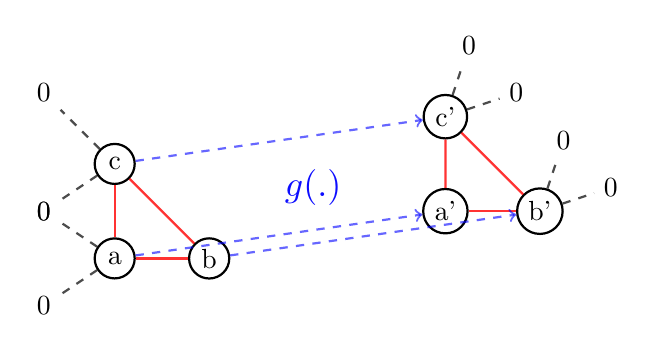
\begin{tikzpicture}[scale=0.6]
          \tikzstyle{every node} = [draw, circle, inner sep = 2pt, thick, minimum size=0.2in];
          \node(1) at (0,0) {a};
          \node(2) at (2,0) {b};
          \node(3) at (0,2) {c};

          \node(4) at (7,1) {a'};
          \node(5) at (9,1) {b'};
          \node(6) at (7,3) {c'};

          \path[opacity=0.8,thick,red] (1) edge (2);
          \path[opacity=0.8,thick,red] (1) edge (3);
          \path[opacity=0.8,thick,red] (2) edge (3);

          \path[opacity=0.8,thick,red] (4) edge (5);
          \path[opacity=0.8,thick,red] (4) edge (6);
          \path[opacity=0.8,thick,red] (5) edge (6);

          \tikzstyle{every node} = []
          \node(7) at (-1.5,3.5) {\h{0}};
          \path[opacity=0.7,thick, dashed] (3) edge (7); 
          \node(8) at (-1.5, 1) {\h{0}};
          \path[opacity=0.7,thick, dashed] (3) edge (8);

          \node(9) at (-1.5,1) {\h{0}};
          \path[opacity=0.7,thick, dashed] (1) edge (9); 
          \node(10) at (-1.5, -1) {\h{0}};
          \path[opacity=0.7,thick, dashed] (1) edge (10);

          \node(13) at (8.5,3.5) {\h{0}};
          \path[opacity=0.7,thick, dashed] (6) edge (13); 
          \node(14) at (7.5,4.5) {\h{0}};
          \path[opacity=0.7,thick, dashed] (6) edge (14);

          \node(17) at (10.5,1.5) {\h{0}};
          \path[opacity=0.7,thick, dashed] (5) edge (17); 
          \node(18) at (9.5,2.5) {\h{0}};
          \path[opacity=0.7,thick, dashed] (5) edge (18);

          \path[opacity=0.6,thick,dashed,->,blue] (1) edge (4);
          \path[opacity=0.6,thick,dashed,->,blue] (2) edge (5);
          \path[opacity=0.6,thick,dashed,->,blue] (3) edge (6);
          \node[opacity=0.95] at (4.2,1.5) {\scalebox{1.3}{$\textcolor{blue}{g(.)}$}};
          \end{tikzpicture}
    \end{center}
    \caption{Local depiction of the action of an LP convolution. The supporting set (red) is moved under the action of $g(.)$ to a subgraph of same shape.}
    \label{fig:lp}
  \end{figure}

Similarly than with EC and EC*, we are also interested to particularize this property for operators with small kernels.

\begin{definition}\textbf{Strictly locality-preserving convolution operator}\\
We say that a $\varphi$-convolution operator, of supporting set $\cm \subset \Gamma$, is strictly locality-preserving (LP*) if every subgraph  $\ck_u = g_u(\ck_e)$ are isomorphic.
\label{def:lpp}
\end{definition}

\begin{remark}
We assume that $\M$-convolution operator are always LP* in the sense that the sum is always over $\cm$. Also note that LP is a stronger property than LP* (\ie LP implies LP*) and that LP* and LP are not related in the same way than EC* and EC.
\end{remark}

Similarly than for EC convolutions, LP convolutions can be characterized with Cayley subgraphs.

\begin{lemma}
On left Cayley graphs, right multiplicative auto-actions are automorphisms (and vice-versa).
\label{lem:lat}
\end{lemma}
\begin{proof}
Since $a \rightarrow b \Leftrightarrow \exists g, ga = b \Leftrightarrow \exists g, gah = bh \Leftrightarrow ah \rightarrow bh$.
\end{proof}

\begin{theorem}\textbf{LP characterization by Cayley subgraphs}\\
Let a graph $\gve$,
\begin{enumerate}[nolistsep,noitemsep,label=(\roman*)]
\item its right Cayley subgraphs characterize its LP $\varphi$-convolutions
\item its abelian Cayley subgraphs characterize its LP $\M$-convolutions
\end{enumerate}
\label{th:cayleycharLP}
\end{theorem}
\begin{proof}
%By using \lemref{lem:lat} and reducing to Sabidussi's theorem: "A graph $G$ is a Cayley graph of a group $\Gamma$ if and only if it admits a simply transitive action of $\Gamma$ by graph automorphisms" (\cite{sabidussi1958class,wiki:cayley}).
Let a group $\Gamma$ of generating set $\cu$. Denote $\vec{G^R}$ the right Cayley graph and $\vec{G^L}$ the left one. Let us assume that $\Gamma \overset\varphi\equiv V$. We denote the action corresponding to the usual left equivalence by $g^L(.) = \varphi \circ L_g \circ \varphi^{-1}$, and the action corresponding to the right equivalence by $g^R(.) = \varphi \circ R_g \circ \varphi^{-1}$, where $L$ and $R$ are the left and right multiplicative auto-actions by $\Gamma$ on itself, as in \eqref{eq:PP} and \eqref{eq:PPPP}. By \lemref{lem:lat}, $g^L(.)$, that is EC on $\vec{G^L}$, is LP on $\vec{G^R}$, and vice-versa. By \thref{th:cayleychar}, $\vec{G^L}$ characterizes $g^L(.)$, while naturally also characterizing $\vec{G^R}$. Therefore, $\vec{G^R}$ characterizes $g^L(.)$, onto which it is LP, so is the corresponding $\varphi$-convolution.
\end{proof}

\begin{corollary}\textbf{Characterization of convolutions that are EC and LP}\\
Let a graph $\gve$, 
\begin{enumerate}[nolistsep,noitemsep,label=(\roman*)]
\item if a $\varphi$-convolution of group $\Gamma$ is EC and LP then $\Gamma$ is abelian,
\item an $\M$-convolution is EC if, and only if, it is also LP.
\end{enumerate}
\label{cor:cayleycharECLP}
\end{corollary}
\begin{proof}
As a consequence of \thref{th:cayleychar} and \thref{th:cayleycharLP}.
\end{proof}

\subsection{Checkpoint summary}

In \secref{sec:2.2}, we obtained two formulations of convolutions of signals on a graph $\gve$, $\ast_\varphi$ and $\ast_{\M}$, depending on a group $\Gamma$, that preserve fully the characterization by equivariance to actions of $\Gamma$. The $\varphi$-convolution can be used given a bijective equivariant map $\varphi$ between $\Gamma$ and a subset $V_s \subset V$, whereas the $\M$-convolution can be used under the condition that $\Gamma$ is abelian. Then in \secref{sec:edges}, we introduced conditions related to the edge set $E$, which leads us to define EC and LP convolutions, that we were able to characterize by Cayley subgraph isomorphism, and for which we were capable to understand the impact of abelianity. We also defined EC* and LP* convolution operators, that are closer to what can be used in deep learning practice. In particular, to define an EC* convolution operator, we only need to search for a set of actions that is a generating set of $\Gamma$. A practical example will be seen in \secref{sec:trans}.

The sets of theorems we obtained are already satisfactory enough to understand how to convolute signals on any graph, using symmetries defined by a group acting on the vertex domain (or on a subset of the vertex domain). Therefore we can consider that the main contributions of this chapter have already been presented.

Nonetheless, symmetries defined by groups can have limitations, since they may be too perfect for some graphs, as discussed in the next section. Hence, we can try to extend further the construction with partial symmetries defined by groupoids. That is the research avenue that we explore in the remainder of this chapter.